\documentclass{lecturenotes}

\title[Kort presentation av PtD \& DoD, 2015-08-27]{EDA016 Programmeringsteknik för D \\ + \\ EDA070 Datorer och datoranvändning}
\author{Björn Regnell \& Roger Henriksson}
\institute{Datavetenskap, LTH}
\date{2015-08-27}
 
\begin{document}
 
\frame{\titlepage}

\SlideImg{Att lägga grunden...}{img/lthgrund.jpg}

\frame{\frametitle{En kurskombo som startar på måndag kl 13:15}
Lägger grunden för alla kommande kurser i datavetenskap: \vspace{1em}
\begin{itemize}
\item Programmeringsteknik för D, 7.5 hp, 16 veckor
\begin{itemize}
\item[] Grundlig genomgång av programmeringens grunder
\end{itemize}
\vspace{1em}
\item Datorer och datoranvändning, 3 hp, 3 veckor
\begin{itemize}
\item[] Inblick i hur datorer fungerar och verktygen vi använder
\end{itemize}
\end{itemize}
}

\frame{\frametitle{Vad ska du lära dig?}
Att skapa koden som styr världen...
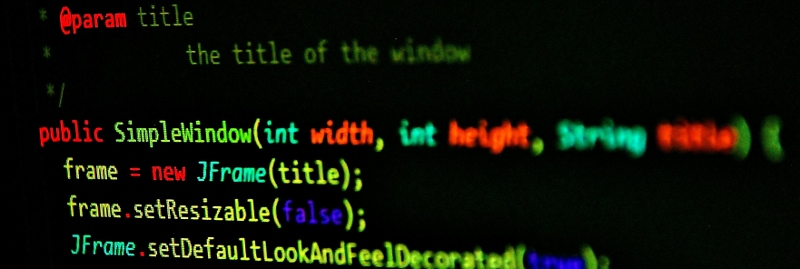
\includegraphics[width=1.2\textwidth, height=1.5cm]{img/code-wide}
\begin{multicols}{2}
\begin{itemize}\Size{9pt}
\item \textbf{Programmeringsteknik för D}
\begin{itemize}\Size{8pt}
\item Programmering från grunden
\item Konstruera algoritmer
\item Tänka i abstraktioner
\item Programspråket Java
\item Utvecklingsmiljön Eclipse
\end{itemize}
\columnbreak
\item \textbf{Datorer \& datoranvändning}
\begin{itemize}\Size{8pt}
\item Lågnivåprogrammering
\item Internet
\item Terminalkommando i Linux
\item Skriva \& typsätta i LaTeX
\item Beräkningar i Matlab
\end{itemize}
\end{itemize}
\end{multicols}
}

%%%
\frame{\frametitle{Hur ska du lära dig?}
\begin{itemize}
\item Genom praktiskt eget arbete: Lära genom att göra!
\item Genom studier av kursteorin: Skapa förståelse
\item Genom samarbete med dina kurskamrater
\end{itemize}
}

\SlideImg{Stor spridning i programmeringsförkunskaper}{img/pre-pie}

%%%
\frame{\frametitle{Förkunskapsenkät}
\begin{itemize}
\item Har du programmerat innan du kom till LTH? \\
         Ja \hspace{2.5cm} Nej
\item Hur många program har du skrivit? \\ 
         $<5$ \hspace{2.2cm} $5-20$ \hspace{2.5cm}  $>20$
\item Hur stort var det största program du har skrivit?\\ 
         $<50$ rader \hspace{1cm} $50 - 500$  rader \hspace{1cm}  $>500$ rader
\end{itemize}
\vspace{1em}
Fyll i denna enkät innan söndag kl 0900:
\url{http://cs.lth.se/eda016/survey}
}

%%%
\frame{\frametitle{Skaffa kurslitteratur på KFS}
\begin{columns}
\begin{column}{0.6\textwidth}
\begin{itemize}
\item ''Objektorienterad programmering och Java" av Per Holm
\item Kurskompendium med övningar och laborationer
\item Bokpaket säljs på KFS \\John Ericssons väg 4 \url{http://www.kfsab.se/}
\end{itemize}
\end{column}
\begin{column}{0.5\textwidth}
\centering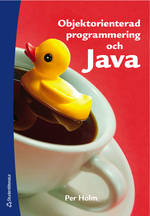
\includegraphics[width=0.5\textwidth]{img/ankbok.jpg}
\end{column}
\end{columns}
}

\SlideImg{Välkommen på måndag kl 13:15 i E:B}{img/ehuset}


\end{document}

